% Options for packages loaded elsewhere
% Options for packages loaded elsewhere
\PassOptionsToPackage{unicode}{hyperref}
\PassOptionsToPackage{hyphens}{url}
\PassOptionsToPackage{dvipsnames,svgnames,x11names}{xcolor}
%
\documentclass[
  letterpaper,
  DIV=11,
  numbers=noendperiod]{scrreprt}
\usepackage{xcolor}
\usepackage{amsmath,amssymb}
\setcounter{secnumdepth}{5}
\usepackage{iftex}
\ifPDFTeX
  \usepackage[T1]{fontenc}
  \usepackage[utf8]{inputenc}
  \usepackage{textcomp} % provide euro and other symbols
\else % if luatex or xetex
  \usepackage{unicode-math} % this also loads fontspec
  \defaultfontfeatures{Scale=MatchLowercase}
  \defaultfontfeatures[\rmfamily]{Ligatures=TeX,Scale=1}
\fi
\usepackage{lmodern}
\ifPDFTeX\else
  % xetex/luatex font selection
\fi
% Use upquote if available, for straight quotes in verbatim environments
\IfFileExists{upquote.sty}{\usepackage{upquote}}{}
\IfFileExists{microtype.sty}{% use microtype if available
  \usepackage[]{microtype}
  \UseMicrotypeSet[protrusion]{basicmath} % disable protrusion for tt fonts
}{}
\makeatletter
\@ifundefined{KOMAClassName}{% if non-KOMA class
  \IfFileExists{parskip.sty}{%
    \usepackage{parskip}
  }{% else
    \setlength{\parindent}{0pt}
    \setlength{\parskip}{6pt plus 2pt minus 1pt}}
}{% if KOMA class
  \KOMAoptions{parskip=half}}
\makeatother
% Make \paragraph and \subparagraph free-standing
\makeatletter
\ifx\paragraph\undefined\else
  \let\oldparagraph\paragraph
  \renewcommand{\paragraph}{
    \@ifstar
      \xxxParagraphStar
      \xxxParagraphNoStar
  }
  \newcommand{\xxxParagraphStar}[1]{\oldparagraph*{#1}\mbox{}}
  \newcommand{\xxxParagraphNoStar}[1]{\oldparagraph{#1}\mbox{}}
\fi
\ifx\subparagraph\undefined\else
  \let\oldsubparagraph\subparagraph
  \renewcommand{\subparagraph}{
    \@ifstar
      \xxxSubParagraphStar
      \xxxSubParagraphNoStar
  }
  \newcommand{\xxxSubParagraphStar}[1]{\oldsubparagraph*{#1}\mbox{}}
  \newcommand{\xxxSubParagraphNoStar}[1]{\oldsubparagraph{#1}\mbox{}}
\fi
\makeatother


\usepackage{longtable,booktabs,array}
\usepackage{calc} % for calculating minipage widths
% Correct order of tables after \paragraph or \subparagraph
\usepackage{etoolbox}
\makeatletter
\patchcmd\longtable{\par}{\if@noskipsec\mbox{}\fi\par}{}{}
\makeatother
% Allow footnotes in longtable head/foot
\IfFileExists{footnotehyper.sty}{\usepackage{footnotehyper}}{\usepackage{footnote}}
\makesavenoteenv{longtable}
\usepackage{graphicx}
\makeatletter
\newsavebox\pandoc@box
\newcommand*\pandocbounded[1]{% scales image to fit in text height/width
  \sbox\pandoc@box{#1}%
  \Gscale@div\@tempa{\textheight}{\dimexpr\ht\pandoc@box+\dp\pandoc@box\relax}%
  \Gscale@div\@tempb{\linewidth}{\wd\pandoc@box}%
  \ifdim\@tempb\p@<\@tempa\p@\let\@tempa\@tempb\fi% select the smaller of both
  \ifdim\@tempa\p@<\p@\scalebox{\@tempa}{\usebox\pandoc@box}%
  \else\usebox{\pandoc@box}%
  \fi%
}
% Set default figure placement to htbp
\def\fps@figure{htbp}
\makeatother





\setlength{\emergencystretch}{3em} % prevent overfull lines

\providecommand{\tightlist}{%
  \setlength{\itemsep}{0pt}\setlength{\parskip}{0pt}}



 


\KOMAoption{captions}{tableheading}
\makeatletter
\@ifpackageloaded{bookmark}{}{\usepackage{bookmark}}
\makeatother
\makeatletter
\@ifpackageloaded{caption}{}{\usepackage{caption}}
\AtBeginDocument{%
\ifdefined\contentsname
  \renewcommand*\contentsname{Table of contents}
\else
  \newcommand\contentsname{Table of contents}
\fi
\ifdefined\listfigurename
  \renewcommand*\listfigurename{List of Figures}
\else
  \newcommand\listfigurename{List of Figures}
\fi
\ifdefined\listtablename
  \renewcommand*\listtablename{List of Tables}
\else
  \newcommand\listtablename{List of Tables}
\fi
\ifdefined\figurename
  \renewcommand*\figurename{Figure}
\else
  \newcommand\figurename{Figure}
\fi
\ifdefined\tablename
  \renewcommand*\tablename{Table}
\else
  \newcommand\tablename{Table}
\fi
}
\@ifpackageloaded{float}{}{\usepackage{float}}
\floatstyle{ruled}
\@ifundefined{c@chapter}{\newfloat{codelisting}{h}{lop}}{\newfloat{codelisting}{h}{lop}[chapter]}
\floatname{codelisting}{Listing}
\newcommand*\listoflistings{\listof{codelisting}{List of Listings}}
\makeatother
\makeatletter
\makeatother
\makeatletter
\@ifpackageloaded{caption}{}{\usepackage{caption}}
\@ifpackageloaded{subcaption}{}{\usepackage{subcaption}}
\makeatother
\usepackage{bookmark}
\IfFileExists{xurl.sty}{\usepackage{xurl}}{} % add URL line breaks if available
\urlstyle{same}
\hypersetup{
  pdftitle={Portofolio M. Abizzar G.},
  pdfauthor={13523155 - M. Abizzar Gamadrian},
  colorlinks=true,
  linkcolor={blue},
  filecolor={Maroon},
  citecolor={Blue},
  urlcolor={Blue},
  pdfcreator={LaTeX via pandoc}}


\title{Portofolio M. Abizzar G.}
\usepackage{etoolbox}
\makeatletter
\providecommand{\subtitle}[1]{% add subtitle to \maketitle
  \apptocmd{\@title}{\par {\large #1 \par}}{}{}
}
\makeatother
\subtitle{Seorang mahasiswa naif yang berusaha menjadi yang terbaik}
\author{13523155 - M. Abizzar Gamadrian}
\date{2025-10-21}
\begin{document}
\maketitle

\renewcommand*\contentsname{Table of contents}
{
\hypersetup{linkcolor=}
\setcounter{tocdepth}{2}
\tableofcontents
}

\bookmarksetup{startatroot}

\chapter*{Selamat Datang di Dunia
Saya}\label{selamat-datang-di-dunia-saya}
\addcontentsline{toc}{chapter}{Selamat Datang di Dunia Saya}

\markboth{Selamat Datang di Dunia Saya}{Selamat Datang di Dunia Saya}

\begin{figure}[H]

{\centering 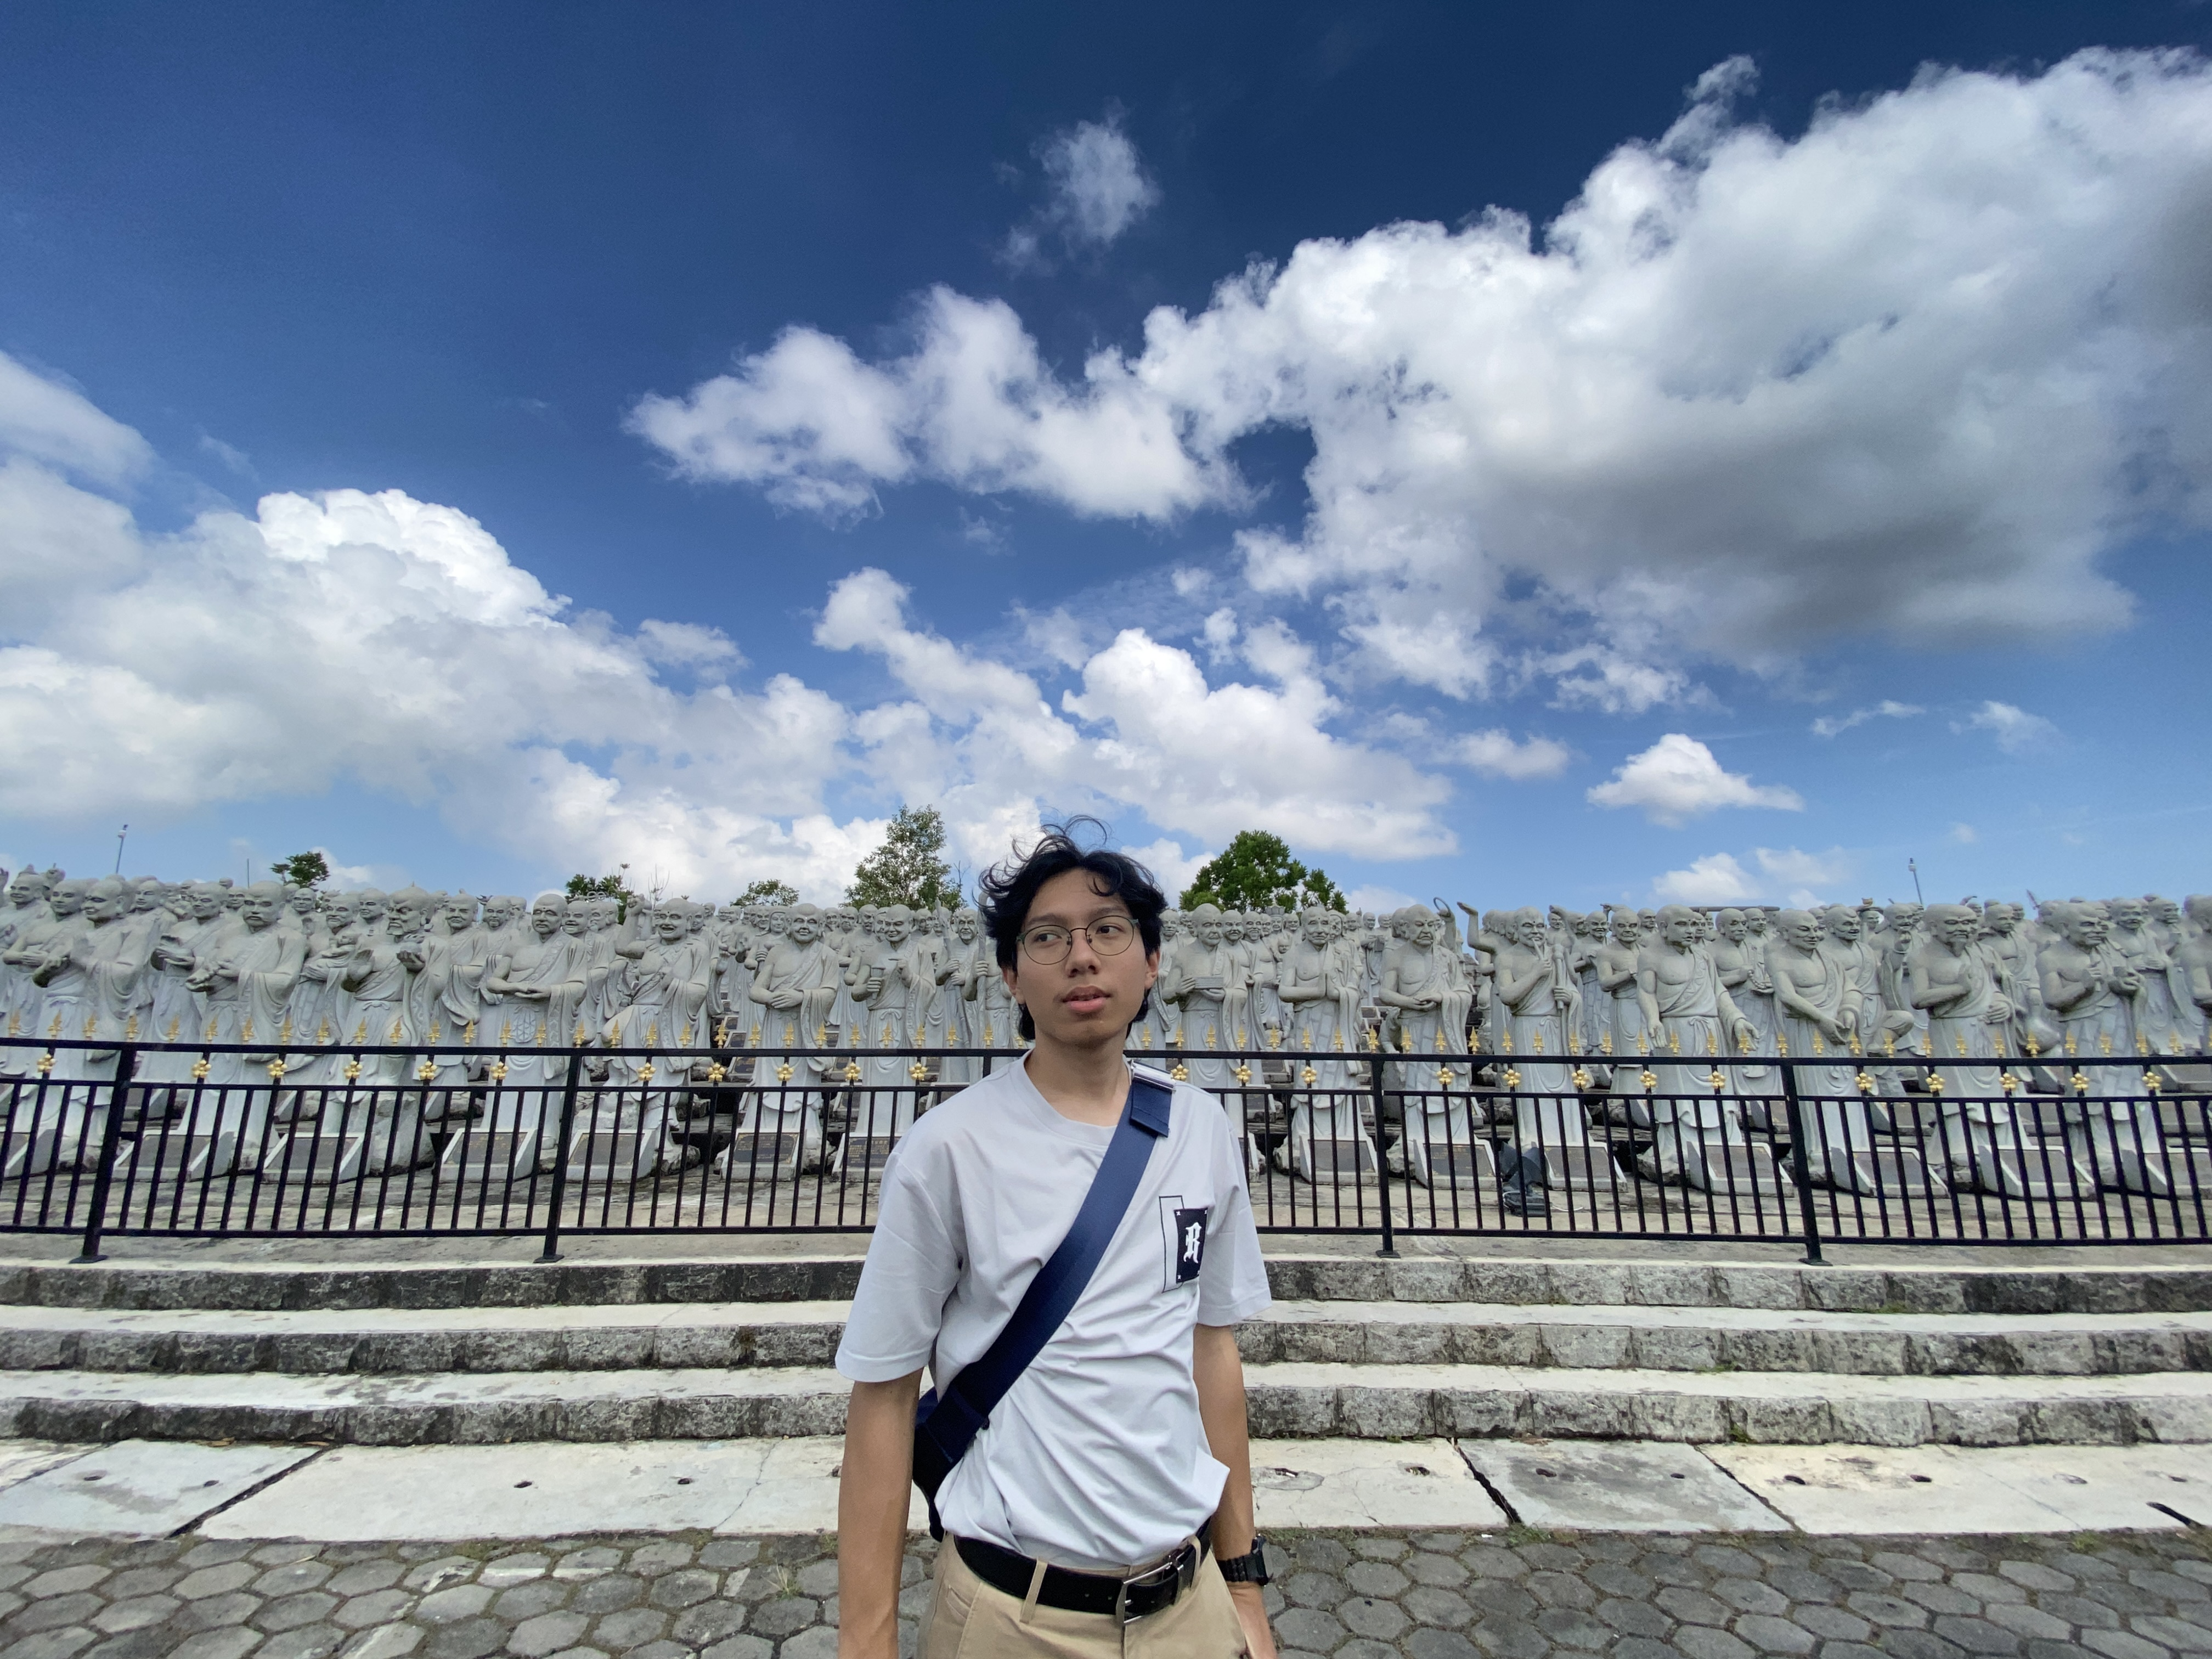
\includegraphics[width=9.5\linewidth,height=\textheight,keepaspectratio]{images/profile.jpg}

}

\caption{Foto M. Abizzar Gamadrian}

\end{figure}%

Selamat datang di portofolio saya. Saya \textbf{M. Abizzar Gamadrian
(13523155)}, dan ini adalah tagline saya: ``seorang mahasiswa naif yang
berusaha menjadi yang terbaik.''

Sesuai tagline itu, halaman ini adalah kumpulan cerita jujur tentang
proses saya---tentang jatuh, bangkit, dan hal-hal aneh di antaranya.

\begin{center}\rule{0.5\linewidth}{0.5pt}\end{center}

\subsection*{Cerita di Balik Sampul (UTS-1: All About
Me)}\label{cerita-di-balik-sampul-uts-1-all-about-me}
\addcontentsline{toc}{subsection}{Cerita di Balik Sampul (UTS-1: All
About Me)}

Untuk mengenal saya, ada beberapa fakta yang perlu Anda tahu:

\begin{enumerate}
\def\labelenumi{\arabic{enumi}.}
\tightlist
\item
  \textbf{Saya buta warna parsial.} Ini bukan halangan, tapi ini membuat
  saya melihat dunia sedikit berbeda (secara harfiah).
\item
  \textbf{Saya punya hobi aneh.} Jika saya bingung menentukan pilihan
  (mau makan apa, nonton apa), saya akan memutar \emph{spin-wheel} di
  internet dan membiarkan takdir memutuskan.
\item
  \textbf{Saya pernah hampir tenggelam.} Waktu kecil, saya nekat mencoba
  menyeberangi kolam yang dalam. Untungnya, sepupu saya melihat dan
  menyelamatkan saya. Mungkin dari situlah saya belajar untuk tidak
  nekat, \emph{atau} setidaknya pastikan ada yang mengawasi.
\end{enumerate}

(Konten UTS-1 selengkapnya ada di chapter
\href{./All_About_me/index.qmd}{All About Me})

\subsection*{Prinsip Saya: Jatuh Itu
Wajar}\label{prinsip-saya-jatuh-itu-wajar}
\addcontentsline{toc}{subsection}{Prinsip Saya: Jatuh Itu Wajar}

Jika ada satu hal yang saya pegang, itu adalah kutipan dari Mary
Pickford:

\begin{quote}
``This thing that we call failure is not the falling down, but the
staying down.''
\end{quote}

Bagi saya, ini bukan sekadar kata-kata. Ini adalah pengingat bahwa gagal
itu tidak apa-apa. Lelah itu wajar. Tapi menyerah? Itu pilihan yang
berbeda. Selama saya tidak memilih untuk ``tetap di bawah'', saya belum
benar-benar gagal.

Prinsip inilah yang membawa saya melewati salah satu kegagalan terbesar
saya, yang bisa Anda baca di \href{./My_Stories_for_You/index.qmd}{My
Stories for You}.

\bookmarksetup{startatroot}

\chapter{UTS-1: All About Me}\label{uts-1-all-about-me}

Halaman ini adalah perpanjangan dari halaman utama. Di luar fakta-fakta
unik dan prinsip hidup, inilah saya di waktu luang.

\subsection{Dunia Saya: Epik dan
Realistis}\label{dunia-saya-epik-dan-realistis}

Saat saya tidak sedang pusing dengan kuliah, saya melarikan diri ke dua
dunia:

\begin{itemize}
\tightlist
\item
  \textbf{Dunia Epik:} Saya fans berat \emph{Attack on Titan}. Bagi
  saya, itu bukan sekadar anime, tapi sebuah mahakarya epik yang akan
  saya rekomendasikan ke semua orang.
\item
  \textbf{Dunia Realistis:} Saya juga sangat menikmati \emph{Better Call
  Saul}.
\end{itemize}

\subsection{Keseimbangan Tubuh dan
Pikiran}\label{keseimbangan-tubuh-dan-pikiran}

Saya bukan tipe orang yang suka lari maraton (aerobik). Saya lebih suka
olahraga anaerobik, secara spesifik \textbf{Calisthenics}. Ada kepuasan
tersendiri dalam melatih kekuatan tubuh.

Dan ya, jika saya sedang penat atau stres karena kuliah, saya suka
bernyanyi-nyanyi. Mungkin tidak merdu, tapi efektif untuk meredakan
stres.

\bookmarksetup{startatroot}

\chapter{UTS-2: Sebuah Lagu Untukmu}\label{uts-2-sebuah-lagu-untukmu}

Pesan ini saya tujukan kepada orang-orang terdekat saya---keluarga dan
sahabat---yang selalu ada bersama saya, bahkan ketika saya melakukan
kesalahan dan belum menjadi yang terbaik.

Saya memilih lagu ``If We Have Each Other'' dari Alec Benjamin.

\subsection{Kenapa Lagu Ini?}\label{kenapa-lagu-ini}

Alasan saya memilih lagu ini sederhana: pesannya sangat kuat. Lagu ini
bercerita bahwa tidak peduli seberapa sulit, kacau, atau tidak
sempurnanya dunia ini, selama kita memiliki satu sama lain, kita akan
baik-baik saja.

Ini adalah janji sekaligus pengingat untuk mereka:

\begin{quote}
``You should know I'll be there for you.''
\end{quote}

Jika mereka sedang kesusahan, mereka harus tahu bahwa saya akan ada
untuk mereka, sama seperti mereka selalu ada untuk saya.

Lirik lagu by Musixmatch:

She was 19 with a baby on the way On the East-side of the city, she was
working every day Cleaning dishes in the evening, she could barely stay
awake She was clinging to the feeling that her luck was gonna change
And, 'cross town she would take the bus at night To a one-bedroom
apartment, and when she'd turn on the light She would sit down at the
table, tell herself that it's alright She was waiting on the day she
hoped her baby would arrive She'd never be alone Have someone to hold
And when nights were cold She'd say The world's not perfect, but it's
not that bad If we got each other, and that's all we have I will be your
mother, and I'll hold your hand You should know I'll be there for you
When the world's not perfect, when the world's not kind If we have each
other, then we'll both be fine I will be your mother, and I'll hold your
hand You should know I'll be there for you They were 90 and were living
out their days On the West-side of the city next to where they got
engaged They had pictures on the walls of all the memories that they'd
made And though life was never easy, they were thankful that they stayed
With each other, and though some times were hard Even when she made him
angry, he would never break her heart No, they didn't have the money to
afford a fancy car But they never had to travel 'cause they'd never be
apart Even at the end Their love was stronger than The day that they
first met They'd say The world's not perfect, but it's not that bad If
we got each other, and that's all we have I will be your lover, and I'll
hold your hand You should know I'll be there for you When the world's
not perfect, when the world's not kind If we have each other, then we'll
both be fine I will be your lover, and I'll hold your hand You should
know I'll be there for you You should know I'll be there for you I'm 23,
and my folks are getting old I know they don't have forever, and I'm
scared to be alone So I'm thankful for my sister, even though sometimes
we fight When high school wasn't easy, she's the reason I survived I
know she'd never leave me and I hate to see her cry So I wrote this
verse to tell her that I'm always by her side I wrote this verse to tell
her that I'm always by her side I wrote this verse to tell her that The
world's not perfect, but it's not that bad If we got each other, and
that's all we have I will be your brother, and I'll hold your hand You
should know I'll be there for you When the world's not perfect, when the
world's not kind If we have each other, then we'll both be fine I will
be your brother, and I'll hold your hand You should know I'll be there
for you You should know I'll be there for you

\bookmarksetup{startatroot}

\chapter{UTS-3: Kisah Gagal di Garis
Start}\label{uts-3-kisah-gagal-di-garis-start}

Kutipan favorit saya tentang kegagalan
\hyperref[uts-3-kisah-gagal-di-garis-start]{di halaman utama} bukan
sekadar teori. Saya mengalaminya.

\subsection{Titik Terendah}\label{titik-terendah}

Momen kegagalan terbesar saya adalah saat pengumuman UTBK. Saya tidak
lulus. Pilihan satu dan pilihan dua, keduanya menolak saya.

Rasanya hancur. Orang tua saya sudah berkorban banyak---menyekolahkan
saya jauh-jauh ke Palembang, ke salah satu SMA terbaik di provinsi,
membiayai kursus tambahan, dan mendukung saya penuh. Tapi saya gagal
memberikan hasil yang membanggakan.

Saya sangat malu. Saya bahkan tidak berani mengabari mereka saat itu.

\subsection{Bukan ``Tetap di Bawah''}\label{bukan-tetap-di-bawah}

Tapi, saya ingat prinsip saya. Saya tidak boleh ``tetap di bawah''.

Orang tua saya, dengan luar biasa, sangat suportif. Mereka tidak marah,
mereka justru mendorong saya untuk mencari jalan lain. Akhirnya, saya
mendaftar dan mengikuti 6 ujian mandiri di berbagai kampus.

Saya tidak membiarkan kesedihan berlarut-larut. Saya tahu saya harus
berjuang lebih keras. Saya percaya Tuhan memberi saya jalan yang
menantang ini karena saya bisa melewatinya. Saya kembali belajar dengan
giat.

\subsection{Hasil}\label{hasil}

Pada akhirnya, saya lulus di 5 dari 6 kampus yang saya daftarkan.

Termasuk di kampus yang awalnya menolak saya di UTBK. Saya
mendapatkannya melalui jalur ujian mandiri, karena saya tidak menyerah
untuk mencoba kembali.

Pelajaran terbesar yang saya dapat adalah validasi dari kutipan itu:

\begin{quote}
``This thing that we call failure is not the falling down, but the
staying down.''
\end{quote}

Jatuh dan tersandung itu hanyalah bagian dari proses yang lebih besar
menuju keberhasilan.

\bookmarksetup{startatroot}

\chapter{UTS-4: Membedah SHAPE Saya}\label{uts-4-membedah-shape-saya}

Di bagian ini, saya melakukan refleksi diri berdasarkan kerangka kerja
SHAPE (Strengths, Heart, Aptitudes, Personality, Experiences). Ini
adalah upaya untuk memahami ``manual'' diri saya sendiri, dengan segala
kelebihan dan kontradiksi menarik di dalamnya.

\subsection{S - Strengths (Kekuatan)}\label{s---strengths-kekuatan}

Saya mengambil asesmen VIA Character Strengths. Hasilnya sangat selaras
dengan apa yang saya rasakan.

\textbf{5 Kekuatan Teratas Saya:} 1. \textbf{Cinta (Love):} Menghargai
hubungan dekat dengan orang lain. 2. \textbf{Perspektif (Perspective):}
Mampu memberikan nasihat bijak. 3. \textbf{Penilaian (Judgment):}
Berpikir kritis dan menimbang dari semua sisi. 4. \textbf{Kejujuran
(Honesty):} Bertindak tulus dan apa adanya. 5. \textbf{Kebaikan
(Kindness):} Senang membantu dan berbuat baik.

\textbf{Refleksi ``Keautentikan'':} Saya sangat setuju dengan 5 kekuatan
teratas ini. Kekuatan \textbf{Cinta (Love)}, \textbf{Kebaikan
(Kindness)}, dan \textbf{Kejujuran (Honesty)} adalah fondasi saya. Saya
selalu berusaha jujur, yang terbukti sejak dulu saat saya memilih untuk
juara kelas 100\% tanpa mencontek. Mencapai sesuatu dengan jujur terasa
jauh lebih memuaskan.

Kekuatan \textbf{Perspektif} dan \textbf{Penilaian} juga sangat ``saya
banget''. Ini terhubung langsung dengan bakat saya sebagai pendengar
yang baik; saya tidak hanya mendengar, tetapi juga mencoba memberikan
perspektif baru atas masalah yang diceritakan teman saya.

\subsection{H - Heart (Hati: Nilai \&
Gairah)}\label{h---heart-hati-nilai-gairah}

Hasil tes Personal Values saya menunjukkan 5 nilai teratas yang memandu
hidup saya: 1. \textbf{Certainty (Kepastian):} Saya menyukai stabilitas,
keteraturan, dan prediktabilitas. Saya merasa nyaman dan aman ketika
segala sesuatunya jelas. 2. \textbf{Financial Stability (Stabilitas
Finansial):} Bagi saya, uang adalah instrumen untuk memenuhi kebutuhan
dan mimpi. Saya sangat rapi dalam mengelola keuangan bulanan untuk
mencapai ini. 3. \textbf{Success (Sukses):} Mencapai hasil yang
diinginkan adalah konfirmasi bahwa keputusan saya benar, yang membangun
kepuasan dan harga diri. 4. \textbf{Family (Keluarga):} Tempat saya
menemukan cinta, keamanan, dan motivasi. 5. \textbf{Friendship
(Persahabatan):} Saya menghargai ikatan yang kuat, rasa saling percaya,
dan kebersamaan dengan orang-orang baik.

Nilai \textbf{Family} dan \textbf{Friendship} adalah manifestasi nyata
dari kekuatan VIA \#1 saya, yaitu \textbf{Cinta (Love)}.

\subsection{A - Aptitudes (Bakat \&
Keterampilan)}\label{a---aptitudes-bakat-keterampilan}

Ini adalah hal-hal yang saya kuasai, baik secara teknis maupun
interpersonal:

\textbf{Keterampilan Teknis \& Analitis:} * Bisa coding * Bisa mengedit
video (jika ada bahan dan ide) * Pandai mengelola keuangan
pribadi/bulanan dengan rapi * Jago mengingat rute jalan dan arah (tidak
mudah tersesat)

\textbf{Keterampilan Interpersonal (ENFP-style):} * Mudah mengobrol
1-on-1 dengan orang baru * Pandai mendengarkan curhat orang lain
(pendengar yang baik) * Bisa memberikan perspektif baru saat orang lain
bercerita * Jago main game (seringkali membutuhkan strategi dan kerja
sama tim) * Bisa Calisthenics dasar

\subsection{P - Personality
(Kepribadian)}\label{p---personality-kepribadian}

Hasil tes MBTI saya adalah \textbf{ENFP-A (Juru Kampanye)}.

Ini sangat menjelaskan mengapa kekuatan utama saya adalah \textbf{Cinta
(Love)} dan \textbf{Kebaikan (Kindness)}. Sebagai seorang Ekstrovert (E)
dan Perasa (F), saya mendapatkan energi dari interaksi sosial yang
bermakna dan sangat peduli pada hubungan. Ini juga menjelaskan mengapa
saya mudah mengobrol 1-on-1 dan menjadi pendengar yang baik.

\textbf{Refleksi ``Keautentikan'': Paradoks Diri Saya} Hal yang paling
mengejutkan sekaligus paling ``saya banget'' adalah kontradiksi antara
\textbf{Nilai (Heart)} dan \textbf{Kepribadian (Personality)} saya.

\begin{itemize}
\tightlist
\item
  Nilai \#1 saya adalah \textbf{Certainty (Kepastian)}. Saya suka hal
  yang jelas dan terencana.
\item
  Tapi, hasil MBTI saya menunjukkan saya 63\% \textbf{Improvising
  (Prospecting/P)}, yang artinya saya lebih dominan improvisasi daripada
  perencanaan kaku.
\end{itemize}

Refleksi saya adalah: Saya adalah seorang \textbf{``Improviser yang
Mencari Kepastian''}. Saya tidak suka rencana yang kaku, tapi saya
\emph{butuh} tujuan yang pasti. Saya mungkin fleksibel dan jago
improvisasi \emph{dalam perjalanan}, tapi saya harus tahu \emph{ke mana}
saya akan pergi (Finansial Stabil, Sukses, dll). Ini adalah inti dari
diri saya: Fleksibel dalam cara, namun pasti dalam tujuan.

\subsection{E - Experiences
(Pengalaman)}\label{e---experiences-pengalaman}

Dua pengalaman hidup ini sangat membentuk saya: 1. \textbf{Juara Kelas
dengan Kejujuran:} Saat sekolah, saya pernah juara kelas 100\% jujur
tanpa mencontek. Pengalaman itu menanamkan nilai bahwa
\textbf{Kejujuran} (kekuatan VIA saya) jauh lebih memuaskan daripada
pencapaian instan lewat kebohongan. 2. \textbf{Orang Datang dan Pergi:}
Saya dulu sering punya teman yang sangat dekat, namun seiring
berjalannya waktu, hubungan itu memudar bukan karena konflik, tapi
karena keadaan dan kesibukan. Ini mengajarkan saya pelajaran berharga:
\emph{``It's okay that people come and go.''} Ini membuat saya semakin
menghargai \textbf{Keluarga} dan \textbf{Persahabatan} (nilai saya) yang
bertahan \emph{saat ini}.

\begin{center}\rule{0.5\linewidth}{0.5pt}\end{center}

\subsection{Piagam Diri (Self Charter)
Saya}\label{piagam-diri-self-charter-saya}

Berdasarkan semua analisis SHAPE ini, inilah Piagam Diri saya:

\begin{quote}
``Saya adalah \textbf{Juru Kampanye (ENFP)} yang beroperasi dengan inti
\textbf{Cinta (Love)} dan \textbf{Kejujuran (Honesty)}.

Kekuatan saya terletak pada kemampuan untuk \textbf{terhubung
(Kindness)} dengan orang lain dan memberikan \textbf{Perspektif
(Perspective)} yang jernih.

Saya adalah paradoks yang hidup: seorang \textbf{improviser (P)} yang
mendambakan \textbf{kepastian (Certainty)}. Saya fleksibel dalam metode,
tapi teguh pada nilai.

Saya dibentuk oleh \textbf{kegagalan (UTS-3)} dan \textbf{persahabatan},
yang mengajarkan saya bahwa jatuh itu wajar, dan bahwa orang boleh
datang dan pergi.

Tujuan saya adalah meraih \textbf{Sukses} dan \textbf{Stabilitas
Finansial} sambil tetap menjadi pendengar yang baik bagi
\textbf{Keluarga} dan \textbf{Sahabat} saya.''
\end{quote}

\bookmarksetup{startatroot}

\chapter{UTS-5 My Personal Reviews}\label{uts-5-my-personal-reviews}

Berikut adalah hasil self-assessment portofolio saya. Metode ini
mengikuti panduan tugas, di mana saya (sebagai penilai) menganalisis
karya saya sendiri menggunakan rubrik yang telah disediakan.

\bookmarksetup{startatroot}

\chapter{Hasil Self-Assessment UTS (URL:
https://abizzarg.github.io/all-about-me/)}\label{hasil-self-assessment-uts-url-httpsabizzarg.github.ioall-about-me}

\section{Identifikasi}\label{identifikasi}

\begin{itemize}
\tightlist
\item
  \textbf{Nama \& NIM penulis:} M. Abizzar Gamadrian -- 13523155
  (tertera di halaman depan portofolio).
\item
  \textbf{Penilai:} Self-assessment (M. Abizzar Gamadrian)
\item
  \textbf{Catatan cakupan:} Halaman beranda (\texttt{index.qmd}) memuat
  rangkuman ``About Me'' (UTS-1) dan ``Prinsip Saya'' (terhubung ke
  UTS-3). Navigasi di \emph{sidebar} lengkap ke semua chapter (UTS-1 s/d
  UTS-5).
\end{itemize}

\section{Tinjauan Umum}\label{tinjauan-umum}

\begin{itemize}
\tightlist
\item
  \textbf{UTS-1 (All About Me)} hadir di chapter
  \texttt{All\_About\_me/index.qmd} dan \texttt{index.qmd}. Konten
  sangat personal, memperkenalkan fakta unik (buta warna, spin-wheel),
  hobi (AoT, calisthenics), dan prinsip hidup (``staying down'').
\item
  \textbf{UTS-2 (My Songs for You)} memuat dedikasi yang jelas, video
  YouTube yang di-embed, narasi personal di balik pemilihan lagu, serta
  lirik lengkap. Konten sudah 100\% lengkap.
\item
  \textbf{UTS-3 (My Stories for You)} berisi satu narasi kuat tentang
  pengalaman kegagalan UTBK, dengan struktur cerita (konflik, resolusi)
  yang jelas.
\item
  \textbf{UTS-4 (My SHAPE)} berisi analisis komprehensif (S-H-A-P-E),
  menghubungkan data tes (VIA, ENFP, Values) dengan refleksi otentik
  (paradoks ENFP vs Certainty) dan ditutup Piagam Diri.
\item
  \textbf{UTS-5 (My Personal Reviews)} (halaman ini) berisi
  \emph{self-assessment} sesuai format. Bagian \emph{Peer-Assessment}
  akan ditambahkan kemudian.
\end{itemize}

\begin{center}\rule{0.5\linewidth}{0.5pt}\end{center}

\section{Tinjauan Spesifik + Skor
(1--5)}\label{tinjauan-spesifik-skor-15}

\subsection{UTS-1 --- All About Me}\label{uts-1-all-about-me-1}

\textbf{Skor per kriteria:} Orisinalitas \textbf{5}, Keterlibatan
\textbf{5}, Humor \textbf{4}, Wawasan/Insight \textbf{5} → \textbf{Total
19/20 (95\%)}. \textbf{Alasan singkat:} Konten sangat otentik dan tidak
kaku. Penggunaan fakta unik (spin-wheel) memenuhi kriteria ``Humor''.
Penggunaan kutipan ``staying down'' sebagai benang merah portofolio
menunjukkan ``Wawasan'' yang kuat. \textbf{Saran perbaikan:} Konten
UTS-1 sedikit terbagi antara \texttt{index.qmd} (Halaman Utama) dan
\texttt{All\_About\_me/index.qmd}. Pertimbangkan untuk menyatukan semua
teks perkenalan diri di dalam chapter \texttt{All\_About\_me/index.qmd}
agar lebih runut.

\subsection{UTS-2 --- My Songs for You}\label{uts-2-my-songs-for-you}

\textbf{Skor per kriteria:} Orisinalitas \textbf{4}, Keterlibatan
\textbf{5}, Humor \textbf{1}, Inspirasi \textbf{5} → \textbf{Total 15/20
(75\%)}. \textbf{Alasan singkat:} ``Keterlibatan'' dan ``Inspirasi''
sangat tinggi karena adanya narasi personal ``kenapa lagu ini''.
Penggunaan \emph{embed} video lebih baik daripada link mati. Skor
``Orisinalitas'' 4 (bukan 5) karena menggunakan karya orang lain (bukan
ciptaan sendiri). Skor ``Humor'' 1 karena pesan lagu ini memang tidak
ditujukan untuk lucu. Konten sekarang sudah lengkap dengan transkrip
lirik, membuat pesan tersampaikan dengan utuh. \textbf{Saran perbaikan:}
Tidak ada. Konten sudah lengkap.

\subsection{UTS-3 --- My Stories for
You}\label{uts-3-my-stories-for-you}

\textbf{Skor per kriteria:} Orisinalitas \textbf{5}, Keterlibatan
\textbf{5}, Pengembangan Narasi \textbf{5}, Inspirasi \textbf{5} →
\textbf{Total 20/20 (100\%)}. \textbf{Alasan singkat:} Cerita kegagalan
UTBK sangat personal, jujur (``malu mengabari orang tua''), dan memenuhi
rubrik ``Pengembangan Narasi'' (Setup: gagal, Conflict: malu \&
berjuang, Resolution: lulus 5/6). Poin ``Inspirasi'' maksimal karena
terhubung langsung dengan tema utama portofolio (``staying down'').
\textbf{Saran perbaikan:} Sudah sangat kuat. Tidak ada perbaikan mayor.

\subsection{UTS-4 --- My SHAPE}\label{uts-4-my-shape}

\textbf{Skor per kriteria:} Orisinalitas \textbf{5}, Keterlibatan
\textbf{5}, Keautentikan \textbf{5}, Inspirasi \textbf{5} →
\textbf{Total 20/20 (100\%)}. \textbf{Alasan singkat:} Ini adalah bagian
terkuat. Skor ``Keautentikan'' maksimal karena tidak hanya melaporkan
hasil tes, tetapi menganalisis paradoks (ENFP vs Certainty).
``Orisinalitas'' tinggi karena menghubungkan semua data (VIA, Aptitudes,
Experiences) menjadi ``Piagam Diri'' yang koheren. \textbf{Saran
perbaikan:} Untuk meningkatkan ``Keterlibatan'' visual, pertimbangkan
membuat 1 tabel ringkas di bagian atas yang merangkum hasil S-H-A-P-E
sebelum masuk ke narasi reflektif.

\subsection{UTS-5 --- My Personal
Reviews}\label{uts-5-my-personal-reviews-1}

\textbf{Skor per kriteria:} Pemahaman Konsep \textbf{5}, Analisis Kritis
\textbf{4}, Argumentasi (Logos) \textbf{4}, Etos \& Empati \textbf{N/A},
Rekomendasi \textbf{4} → \textbf{Total (Self-Assess) 17/20 (85\%)}.
\textbf{Alasan singkat:} Halaman ini (saat ini) telah berhasil memenuhi
tugas \emph{Self-Assessment} dengan ``Pemahaman Konsep'' rubrik,
melakukan ``Analisis Kritis'' pada setiap UTS, dan memberikan
``Rekomendasi'' yang spesifik. \textbf{Saran perbaikan:} Tugas ini belum
selesai. Perlu segera dilengkapi dengan: 1. Melakukan
\emph{Peer-Assessment} (menilai 2-3 portofolio rekan) dan menambahkannya
di bawah bagian ini. 2. Mengisi file \texttt{Lembar\ Skor.xlsx}
(termasuk skor \emph{peer-assessment}) dan meng-upload-nya ke folder
ini, lalu membuat \emph{link} unduhan.

\begin{center}\rule{0.5\linewidth}{0.5pt}\end{center}

\section{Rekap Skor (ringkas)}\label{rekap-skor-ringkas}

\begin{itemize}
\tightlist
\item
  \textbf{UTS-1:} 19/20 → \textbf{95\%}
\item
  \textbf{UTS-2:} 15/20 → \textbf{75\%}
\item
  \textbf{UTS-3:} 20/20 → \textbf{100\%}
\item
  \textbf{UTS-4:} 20/20 → \textbf{100\%}
\item
  \textbf{UTS-5:} (Baru Self-Assess) \textbf{17/20 (85\%)}
\end{itemize}

\emph{(Skor ini adalah hasil self-assessment dan akan dilengkapi dengan
Peer-Assessment)}

\section{Langkah Perbaikan Cepat
(Prioritas)}\label{langkah-perbaikan-cepat-prioritas}

\begin{enumerate}
\def\labelenumi{\arabic{enumi}.}
\tightlist
\item
  \textbf{Lengkapi UTS-5:} Ini prioritas utama. Lakukan
  \emph{Peer-Assessment} dan upload \texttt{Lembar\ Skor.xlsx}.
\item
  \textbf{Perbaiki UTS-1:} Satukan konten perkenalan diri ke dalam satu
  chapter \texttt{All\_About\_me/index.qmd}.
\end{enumerate}

\bookmarksetup{startatroot}

\chapter{UAS-1 My Concepts}\label{uas-1-my-concepts}

Mau hidup epik ? \href{lifestory.pdf}{Write your Life Story}

Apa itu berkonsep?

\url{https://youtu.be/QVfUlVBO80U?si=yM6q_rwV9rcDBbu7}

\bookmarksetup{startatroot}

\chapter{UAS-3 My Opinions}\label{uas-3-my-opinions}

SApa itu beropini? \href{BM\%20Opini.mp4}{Opini Berpengaruh}

Bagiamana menjaadi menarik? \href{./Interesting.mp4}{Menjadi Menarik}

\bookmarksetup{startatroot}

\chapter{UAS-3 My Innovations}\label{uas-3-my-innovations}

\bookmarksetup{startatroot}

\chapter{UAS-4 My Knowledge}\label{uas-4-my-knowledge}

Cara saya mengkomunikasikan sebuah pengatahuan sebagai petunjuk bagi
orang lain 1) saya tulis
\href{Rekomendasi\%20Presentasi\%20Efektif(Contoh\%20Makalah).pdf}{makalah
sebagai bahan utama} 2) lalu saya buat
\href{Contoh\%20Transkrip\%20Presentasi.pdf}{transkrip ucapan lisan} 3)
kemudian saya kembangkan
\href{Rekomendasi\%20Presentasi\%20(Contoh\%20Slides).pdf}{slide
pendukung trnsskrip} 4) lalu saya memproduksivideo audio visual
\url{https://youtu.be/ZbghfMvnPZc} \url{https://youtu.be/ZbghfMvnPZc}

\bookmarksetup{startatroot}

\chapter{UAS-5 My Professional
Reviews}\label{uas-5-my-professional-reviews}

Untuk melAkukan review, seperti pada
\href{../My_Personal_Reviews/Doc.5.Mengevaluasi-Esai-Berdasarkan-Rubrik.pdf}{pendekatan
AI}, kita membutuhkan rubrik

\bookmarksetup{startatroot}

\chapter{Summary}\label{summary}

In summary, this book has no content whatsoever.

\bookmarksetup{startatroot}

\chapter*{References}\label{references}
\addcontentsline{toc}{chapter}{References}

\markboth{References}{References}

\phantomsection\label{refs}




\end{document}
